\chapter{Transformata Fouriera: z drgań do widma}\label{rozdz:fourier}

\section{Co jest w tym nagraniu?}

Nagranie to ciąg liczb zmieniających się w czasie. Nas interesuje coś innego: \emph{jakie częstotliwości w nim
grają?} Odpowiada na to transformata Fouriera, która rozkłada sygnał na sinusoidy. Dla krótkiego okna dźwięku
zamienia $N$ próbek w $N$ liczb mówiących, ile energii niesie każda częstotliwość. To jest pierwszy krok liczenia cech
Gen~6 (rozdział~\ref{rozdz:hcqt}). Poznamy jej własności i, co ważne, \emph{ograniczenia}: przeciek i skończoną rozdzielczość.

Po tym rozdziale umiesz: (i)~policzyć DFT małego sygnału ręcznie, (ii)~uzasadnić, że wiąże ona sinusoidy z pojedynczymi prążkami,
(iii)~wyjaśnić, czemu stosuje się okno Hanna, (iv)~policzyć rozdzielczość $f_s/N$ i ocenić, czy dwa dźwięki da się rozdzielić.

\section{Liczby zespolone w dwóch zdaniach}

\haslo{wzór Eulera}
\begin{definicja}[Jednostka urojona i wzór Eulera]\label{def:euler}
Liczba $i$ spełnia $i^2=-1$. Dla rzeczywistego $\theta$ definiujemy
$e^{i\theta}=\cos\theta+i\sin\theta$ --- punkt na okręgu jednostkowym o kącie $\theta$.
Moduł $\abs{a+ib}=\sqrt{a^2+b^2}$. Zachodzi $e^{i\alpha}e^{i\beta}=e^{i(\alpha+\beta)}$ oraz $\abs{e^{i\theta}}=1$.
\end{definicja}

\begin{przyklad}\label{prz:euler}
$e^{i\pi}=\cos\pi+i\sin\pi=-1$, $e^{i\pi/2}=i$, $e^{-i\pi/2}=-i$. Zatem
$\cos\theta=\tfrac12(e^{i\theta}+e^{-i\theta})$ i $\sin\theta=\tfrac1{2i}(e^{i\theta}-e^{-i\theta})$ --- sinus i cosinus to
„składowe” punktu na okręgu.
\end{przyklad}

\section{Dyskretna transformata Fouriera}

\haslo{DFT}
\begin{definicja}[DFT]\label{def:dft}
Dla ciągu $x[0],\dots,x[N-1]$ jego \emph{dyskretna transformata Fouriera} to ciąg liczb zespolonych
\begin{equation}
  X[k]=\sum_{n=0}^{N-1}x[n]\,e^{-2\pi i\,kn/N},\qquad k=0,1,\dots,N-1.
  \label{eq:dft}
\end{equation}
Numer $k$ odpowiada częstotliwości $f_k=k\,f_s/N$; $\abs{X[k]}$ nazywamy \emph{widmem amplitudowym}.
Odstęp $\Delta f=f_s/N$ między sąsiednimi $k$ to \emph{rozdzielczość} (szerokość binu) DFT.
\end{definicja}

\begin{przyklad}[$N=4$ ręcznie]\label{prz:dft4}
Niech $x=(1,0,-1,0)$, czyli jeden okres cosinusa w $4$ próbkach. Ponieważ $e^{-2\pi ikn/4}=(-i)^{kn}$:
$X[0]=1+0-1+0=0$; $X[1]=1+(-1)(-i)^{2}=1+1=2$; $X[2]=1+(-1)(-i)^{4}=1-1=0$; $X[3]=1+(-1)(-i)^{6}=1+1=2$.
Widmo $\abs{X}=(0,2,0,2)$: cosinus daje dwa prążki, w $k=1$ i lustrzany $k=3=N-1$. Przy $f_s=4\Hz$ prążek $k=1$ to $1\Hz$.
\end{przyklad}

\begin{intuicja}
$X[k]$ mierzy, jak bardzo sygnał „zgadza się” z sinusoidą o $k$ obiegach na okno: mnożymy sygnał przez tę sinusoidę i
sumujemy (to iloczyn skalarny z rozdziału~\ref{rozdz:wektory}!). Gdy sygnał ją zawiera, wszystkie składniki sumy dodają się;
gdy nie, wzajemnie się znoszą.
\end{intuicja}

\begin{twierdzenie}[Ortogonalność sinusoid]\label{tw:ortogonalnosc}
Dla całkowitych $k,l$:
\begin{equation}
  \sum_{n=0}^{N-1}e^{2\pi i(k-l)n/N}=\begin{cases}N,&k\equiv l\pmod N,\\0,&\text{w przeciwnym razie.}\end{cases}
\end{equation}
\end{twierdzenie}
\begin{pomyslDowodu}
To suma wyrazów ciągu geometrycznego o ilorazie $q=e^{2\pi i(k-l)/N}$, a $q^N=1$.
\end{pomyslDowodu}
\begin{proof}
Niech $q=e^{2\pi i(k-l)/N}$. Gdy $k\equiv l\pmod N$, to $q=1$ i suma ma $N$ składników równych $1$, czyli wynosi $N$.
W przeciwnym razie $q\neq1$ i ze wzoru na sumę ciągu geometrycznego
\begin{align*}
\sum_{n=0}^{N-1}q^n &= \frac{1-q^N}{1-q} && \pow{(suma geometryczna)}\\
 &= \frac{1-e^{2\pi i(k-l)}}{1-q}=\frac{1-1}{1-q}=0. && \pow{($q^N=e^{2\pi i(k-l)}=1$)}
\end{align*}
Sinusoidy o różnych numerach są więc wzajemnie prostopadłe (iloczyn skalarny zero), a o tym samym mają „długość” $\sqrt N$. To kończy dowód.
\end{proof}

\begin{wniosek}[DFT sinusoidy o całkowitej liczbie okresów]\label{wn:dft-cos}
Jeśli $x[n]=A\cos(2\pi k_0n/N)$ dla całkowitego $0<k_0<N/2$, to $X[k_0]=X[N-k_0]=AN/2$, a pozostałe $X[k]=0$.
\end{wniosek}
\begin{proof}
Z przykładu~\ref{prz:euler}: $x[n]=\tfrac A2\big(e^{2\pi ik_0n/N}+e^{-2\pi ik_0n/N}\big)$. Wstawiamy do \eqref{eq:dft}:
\begin{align*}
X[k] &= \frac A2\sum_{n}e^{2\pi i(k_0-k)n/N}+\frac A2\sum_{n}e^{-2\pi i(k_0+k)n/N} && \pow{(rozdzielność)}\\
     &= \frac A2\,N\,\indic{k=k_0}+\frac A2\,N\,\indic{k=N-k_0}. && \pow{(tw.~\ref{tw:ortogonalnosc})}
\end{align*}
Dla $N=4$, $k_0=1$, $A=1$ daje to $X[1]=X[3]=2$, zgodnie z przykładem~\ref{prz:dft4}. Czysty ton daje więc dokładnie jeden prążek (i jego lustro).
\end{proof}

\section{Przeciek i okno}

Jest haczyk: wniosek~\ref{wn:dft-cos} wymaga, by ton miał \emph{całkowitą} liczbę okresów w oknie. Częstotliwości
nut tego nie spełniają. Co się dzieje, gdy $k_0$ nie jest całkowite?

\begin{twierdzenie}[Przeciek]\label{tw:przeciek}
Niech $x[n]=e^{2\pi i\,\kappa n/N}$ z dowolnym rzeczywistym $\kappa$ i niech $\delta=\kappa-k$. Wtedy
\begin{equation}
  \abs{X[k]}=\left|\frac{\sin(\pi\delta)}{\sin(\pi\delta/N)}\right|.
\end{equation}
Jest to $N$ dla $\delta=0$, zero dla niezerowych całkowitych $\delta$ i ok.\ $\frac{2}{\pi}N\approx0{,}64N$ dla $\delta=\tfrac12$
(dla dużych $N$).
\end{twierdzenie}
\begin{pomyslDowodu}
To znów suma geometryczna, tym razem z ilorazem $e^{2\pi i\delta/N}\neq1$; moduł licznika i mianownika daje sinusy.
\end{pomyslDowodu}
\begin{proof}
Z \eqref{eq:dft} i definicji $\delta$:
\begin{align*}
X[k] &= \sum_{n=0}^{N-1}e^{2\pi i\delta n/N}=\frac{1-e^{2\pi i\delta}}{1-e^{2\pi i\delta/N}} && \pow{(suma geometryczna)}\\
 &= \frac{e^{i\pi\delta}\,(e^{-i\pi\delta}-e^{i\pi\delta})}{e^{i\pi\delta/N}\,(e^{-i\pi\delta/N}-e^{i\pi\delta/N})} && \pow{(wyłączenie połówek kątów)}\\
 &= e^{i\pi\delta(1-1/N)}\,\frac{\sin(\pi\delta)}{\sin(\pi\delta/N)}. && \pow{(wzór Eulera na sinus)}
\end{align*}
Moduł czynnika $e^{i\cdots}$ wynosi $1$, więc zostaje podany wzór. Dla $\delta=0$ granica to $N$; dla całkowitego $\delta\neq0$ licznik jest zerem; dla $\delta=\frac12$ mianownik $\sin(\pi/2N)\approx\pi/2N$, a licznik $1$, czyli $\approx2N/\pi$. To kończy dowód.
\end{proof}

W zwykłym języku: ton między binami „rozlewa się” na sąsiednie prążki i traci w najgorszym miejscu ok.\ $3{,}9\dB$ głośności ($20\log_{10}(2/\pi)=-3{,}9\dB$). Poza tym ogony przecieku opadają wolno: pierwszy listek boczny okna prostokątnego to tylko $-13\dB$.
Silny ton zasłoni więc słabe składowe daleko od siebie. Rozwiązaniem jest okno.

\haslo{okno Hanna}
\begin{definicja}[Okno Hanna]\label{def:hann}
\emph{Oknem Hanna} nazywamy $w[n]=\tfrac12\big(1-\cos(2\pi n/N)\big)$, $n=0,\dots,N-1$. Przed liczeniem DFT mnożymy próbki przez $w[n]$.
\end{definicja}

\begin{przyklad}\label{prz:hann}
Dla $N=8$: $w=(0;\,0{,}146;\,0{,}5;\,0{,}854;\,1;\,0{,}854;\,0{,}5;\,0{,}146)$: okno łagodnie zaczyna się od zera, osiąga $1$ w środku i znów opada.
Brzegi okna nie są więc ucinane gwałtownie, a to właśnie nagła krawędź powoduje długi ogon przecieku.
\end{przyklad}

\begin{twierdzenie}[Widmo okna Hanna]\label{tw:hann}
Jeśli $Y[k]$ jest DFT sygnału $y[n]$ z oknem prostokątnym, to DFT sygnału $y[n]w[n]$ z oknem Hanna wynosi
$\tfrac12Y[k]-\tfrac14Y[k-1]-\tfrac14Y[k+1]$.
\end{twierdzenie}
\begin{pomyslDowodu}
Zapisujemy $w[n]=\tfrac12-\tfrac14e^{2\pi in/N}-\tfrac14e^{-2\pi in/N}$ i zauważamy, że mnożenie przez $e^{2\pi in/N}$ przesuwa widmo o jeden bin.
\end{pomyslDowodu}
\begin{proof}
Z wzoru Eulera $\cos(2\pi n/N)=\tfrac12\big(e^{2\pi in/N}+e^{-2\pi in/N}\big)$, więc
$w[n]=\tfrac12-\tfrac14e^{2\pi in/N}-\tfrac14e^{-2\pi in/N}$. Dla składnika z $e^{2\pi in/N}$:
\begin{align*}
\sum_n y[n]e^{2\pi in/N}e^{-2\pi ikn/N} &= \sum_n y[n]e^{-2\pi i(k-1)n/N}=Y[k-1]. && \pow{(złączenie wykładników)}
\end{align*}
Analogicznie $e^{-2\pi in/N}$ daje $Y[k+1]$. Z liniowości DFT otrzymujemy podany wzór. To kończy dowód.
\end{proof}

Skutki (to już obserwacja liczbowa, rys.~\ref{rys:przeciek}, a nie część dowodu): kopie z $k\pm1$ mają znak przeciwny niż środkowa, więc
kasują ogon przecieku, a główny listek robi się szerszy ($4$ biny między zerami zamiast $2$). Pierwszy listek boczny
spada z $-13{,}3\dB$ (okno prostokątne) do $-31{,}5\dB$.

\begin{figure*}[ht]
\centering
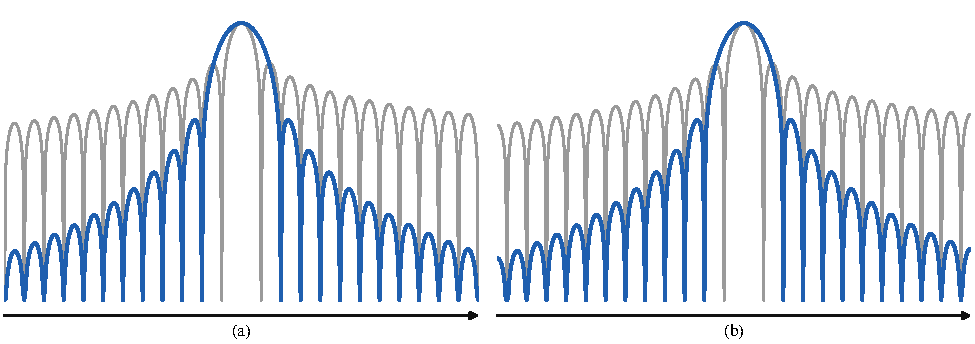
\includegraphics[width=\linewidth]{figures/przeciek.pdf}
\caption{Widmo tonu z $N=128$ próbek w decybelach (skala od $-80$ do $0\dB$, wspólna). Ton dokładnie w prążku (linia ciągła) i w połowie między prążkami (przerywana). (a) Okno prostokątne (szare): wąski pik, ale listki boczne opadają wolno; pierwszy ma $-13\dB$ (pomarańczowa kropkowana). (b) Okno Hanna (niebieskie): pik dwa razy szerszy, ale pierwszy listek tylko $-31\dB$ (pomarańczowa kropkowana), a dalsze opadają szybko. Ton między prążkami ma niższy pik w obu oknach.}
\label{rys:przeciek}
\end{figure*}

\begin{pulapka}
Okno Hanna nie jest za darmo: rozszerza główny listek dwukrotnie, więc \emph{pogarsza rozdzielczość}. Zyskujemy czystość widma
(brak „duchów” od silnych tonów), tracimy zdolność do rozdzielania dwóch bliskich dźwięków. Wybór okna to zawsze kompromis.
\end{pulapka}

\section{Rozdzielczość: kiedy dwa dźwięki są jednym}

Gen~6 liczy FFT dla okna $N=4096$ przy $f_s=11\,025\Hz$ (czas $372\ms$), więc $\Delta f=2{,}69\Hz$; główny listek Hanna ma
$\pm2\Delta f=\pm5{,}4\Hz$. Zero-padding (dopisanie zer, rozdział~\ref{rozdz:hcqt}) dzieli siatkę na $0{,}67\Hz$, ale
\emph{nie zwiększa rozdzielczości} --- tylko interpoluje ten sam kształt.

\begin{naliczbach}
Najniższe nuty gitary leżą blisko siebie: E2 ($82{,}41\Hz$) i F2 ($87{,}31\Hz$) dzieli $4{,}9\Hz$, mniej niż $5{,}4\Hz$ połowy głównego listka.
Numerycznie (rys.~\ref{rys:rozdzielczosc}a) widmo sumy z oknem $4096$ ma dwa „piki” w $84{,}1$ i $85{,}5\Hz$: to artefakt interferencji,
nie prawdziwe położenia nut. Dla E2 i F\#2 ($10{,}1\Hz$ różnicy) piki są już rozdzielone i leżą w $82{,}8$ i $92{,}2\Hz$, czyli mniej niż $0{,}4\Hz$ od prawdy (b).
Okno $N=1024$ ($\Delta f=10{,}8\Hz$) daje dla pary (b) dwa piki w błędnych miejscach ($78{,}1$ i $96{,}9\Hz$).
\end{naliczbach}

\begin{figure*}[ht]
\centering
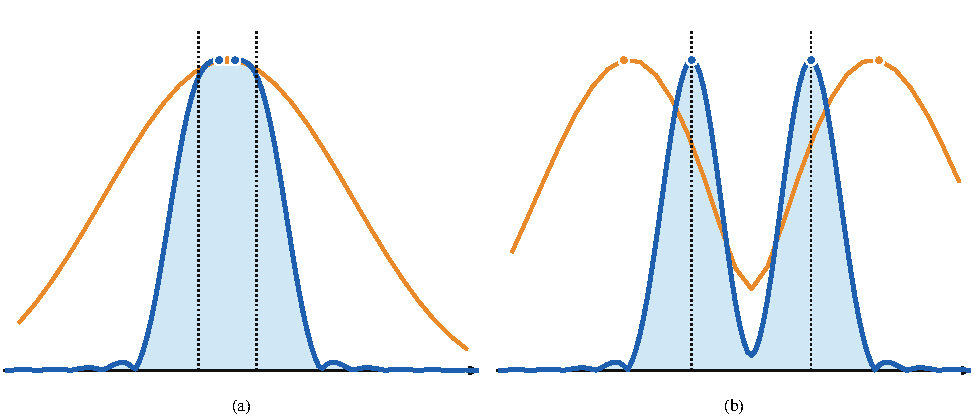
\includegraphics[width=\linewidth]{figures/rozdzielczosc.pdf}
\caption{Widmo (okno Hanna) sumy dwóch sinusoid; czarne kropkowane pionowe linie to prawdziwe częstotliwości, kropki to znalezione piki. Niebieskie z wypełnieniem: okno $N=4096$; pomarańczowe: $N=1024$. (a) E2 i F2 (półton, $4{,}9\Hz$): długie okno daje dwa bliskie piki w złych miejscach (interferencja), krótkie jeden szeroki pagórek. (b) E2 i F\#2 ($10{,}1\Hz$): długie okno rozdziela tony prawie bez błędu położenia, krótkie daje dwa piki odsunięte od prawdy o kilka herców. Dlatego model dostaje dwa okna --- długie dla wysokości, krótkie dla czasu --- i uczy się łączyć wskazówki z wielu klatek.}
\label{rys:rozdzielczosc}
\end{figure*}

Wniosek jest uczciwy i ważny: z samego widma jednej klatki nie da się wiarygodnie odróżnić sąsiednich niskich półtonów.
Dlatego dalsze rozdziały dodają kontekst w czasie (uwaga między klatkami) i szereg alikwotów (wyższe alikwoty są szerzej rozstawione
w hercach, więc łatwiej je rozdzielić).

\section*{Podsumowanie}
\begin{itemize}
\item DFT $X[k]=\sum x[n]e^{-2\pi ikn/N}$; bin $k$ to $kf_s/N$ Hz; rozdzielczość $\Delta f=f_s/N$.
\item Sinusoidy o różnych $k$ są ortogonalne (tw.~\ref{tw:ortogonalnosc}); ton o całkowitej liczbie okresów daje jeden prążek.
\item Ton między binami „przecieka” (tw.~\ref{tw:przeciek}); okno prostokątne ma listki $-13\dB$.
\item Okno Hanna to trzy przesunięte kopie okna prostokątnego (tw.~\ref{tw:hann}): listki $-31\dB$, ale główny listek dwa razy szerszy.
\item Dla $N=4096$ rozdzielczość to $2{,}7\Hz$, a sąsiednie niskie półtony (odstęp $4{,}9\Hz$) nie rozdzielają się czysto.
\end{itemize}

\begin{sprawdz}
\begin{enumerate}
\item Policz ręcznie DFT dla $x=(1,1,0,0)$ ($N=4$) i podaj widmo amplitudowe.
\item Ile wynosi $\Delta f$ dla $N=1024$ i $N=16\,384$ przy $f_s=11\,025\Hz$? Który z nich ma większą \emph{rozdzielczość} i dlaczego $N=16\,384$ z zero-paddingiem z $4096$ nie jest dokładniejszy niż $4096$?
\item Ton $A\cos(2\pi\cdot 10\,n/64)$ ma $N=64$. Które $k$ mają niezerowe $X[k]$ i ile wynosi $\abs{X}$ dla $A=2$?
\item Pokaż, że $\sum_{n=0}^{N-1}w[n]=N/2$ dla okna Hanna (wskazówka: tw.~\ref{tw:ortogonalnosc} z $k=l\pm1$).
\end{enumerate}
\end{sprawdz}

\subsection*{Rozwiązania}
\begin{enumerate}
\item $X[k]=1+e^{-2\pi ik/4}=1+(-i)^k$: $X[0]=2$, $X[1]=1-i$, $X[2]=0$, $X[3]=1+i$. $\abs{X}=(2,\sqrt2,0,\sqrt2)$.
\item $\Delta f=10{,}77\Hz$ i $0{,}673\Hz$. Zero-padding z $4096$ do $16\,384$ daje siatkę $0{,}673\Hz$, ale okno nadal trwa $372\ms$, więc rozdzielczość pozostaje $2{,}69\Hz$ (główny listek tak samo szeroki). Prawdziwe $N=16\,384$ próbek (1,5 s) miałoby $\Delta f=0{,}673\Hz$ \emph{prawdziwej} rozdzielczości.
\item $k=10$ i $k=54$; $\abs{X}=AN/2=2\cdot64/2=64$.
\item $\sum w=\tfrac12N-\tfrac14\sum e^{2\pi in/N}-\tfrac14\sum e^{-2\pi in/N}=\tfrac N2-0-0=\tfrac N2$, bo sumy z $k-l=\pm1$ są zerami.
\end{enumerate}
